%%%%%%%%%%%%%%%%%%%%%%%%%%%%%%%%%%%%%%%%%%%%%%%%%%%%%%%%%%%%%%%
\section{Production and Assembly}
\label{sec:fdsp-pd-prod-assy}
%\metainfo{(Length: TDR=40 pages, TP=8 pages)}

%%%%PHOTON COLLECTORS PRODUCTION %%%%%%%%%%%%%%%%%%%%%%%%%%%%%%%%%%%%%%%%%%%%%%%%%%%
The Single-Phase Photon Collector Consortium is a geographically diverse group of institutions, collaborating across three continents to fabricate a single integrated system.  As such, careful planning and control of component fabrication, assembly and testing must be maintained.

This section describes the planning for fabrication, assembly, and testing, focusing primarily on the PD light collector modules, photosensors and photosensor modules, electronics, and calibration and monitoring.

\subsection{Photon Collector Module Component Fabrication}
The photon detector light collector modules were designed with ease of fabrication in mind.  The module components can be fabricated and tested QC tested at physically separated facilities, later to be collected and assembled at one or more assembly facilities.  Fabrication information for selected components is described below.

\subsubsection{Dichroic filter fabrication and coating, Vikuiti\texttrademark\ reflector foils}

The baseline design for dichroic filters plans for a fused silica plate,  \SI{10}{cm}$\times$\SI{7.8}{cm}$\times$\SI{0.2}{cm}, commercially coated (as described above) to provide for the dichroic properties of the filter.  Our plan for production fabrication envisions continuing to purchase these plates from a commercial vendor (certified by the vendor for performance), and test the performance of a representative sample at a collaboration institution.  

Prior to coating, the filters are cleaned according to the procedures given by the manufacturer using isopropyl alcohol. Since the most likely vector for scratching/damaging the coating is dragging contaminated wipes across the surface, new clean lint free wipes are used for each  cleaning pass on the surface. Clean filters are then baked at 100$^\circ$C for \SI{12}{hours}. 

For \dword{pdsp} \dword{pd} production the evaporation process will be performed at Unicamp in Brazil, where a large vacuum evaporator with an internal diameter of one meter is now available. The conversion efficiency of the film deposited on the filters will be measured for a representative sample, with a dedicated set-up that will use the \SI{127}{nm} light produced by a VUV monochromator.

Vikuiti \texttrademark\ reflector foils required for the rear reflector surface of single-sided X-ARAPUCA supercells and the sides of all modules will be purchased from a vendor, laser-cut to the form factor required by the vendor prior to delivery.  Mechanical and optical QC tests will be performed on a representative sample upon receipt.

\subsubsection{Wavelength shifting plates}

The baseline design for the wavelength shifting plates calls for a plate  composed of Eljen EJ-286 of dimensions \SI{48.7}{cm} $\times$ \SI{93.0}{cm}$\times$ \SI{0.35}{cm}.  The edges of this plate will be simultaneously cut and polished with a diamond-edged cutter to increase internal reflectivity, following a proprietary process developed by Eljen Inc.  Plates will be delivered to the consortium institution responsible for this component, where QC testing of a representative sample will be performed.

\subsubsection{Mechanical components}

The mechanical components comprising the frame of the photon detector modules are primarily fabricated from FR-4 G-10.  This selection was made to mitigate thermal expansion issues (see thermal expansion discussion below), but it imposes difficulties in the manufacturing process, as this material is abrasive and somewhat difficult and expensive to work with using traditional machining processes.

To mitigate these difficulties, most of the photon detector frame components were designed to be amenable to fabrication by means of water-jet cutting processes.  Most components in the design can be fabricated to completion using these techniques.  In the case where post-cutting fabrication are required, typically this is only tapping of pre-cut holes, or (rarely) drilling and tapping holes into the sides of the components where the pilot holes were not able to be pre-cut with the water jet.

Our plan for fabrication calls for procuring water-jet cut components from an external vendor, and conducting secondary fabrication at consortium institution(s) as required.  QC tests of a representative sample of finished components is planned for.

\label{sec:fdsp-pd-prod-pc}
%\metainfo{\color{blue} Content: Warner}

%\fixme{update for x-arapuca}
%\fixme{content to be added}


%%%%ARAPUCA %%%%%%%%
%rjw 20/11/18 No need for subsection with only one light collector!
%\subsubsection{ARAPUCA}
%\label{ssec:fdsp-pd-pc-prod-arapuca}
%\fixme{This section remains to be updated.}
% New from Ana added 8 apr 18

% 12/2/18 rjw This paragraph was in the design section but is more Prod/Assembly so moved here - not sure where to put it though

%Prior to coating, the filters are cleaned according to the procedures given by the manufacturer using isopropyl alcohol. Since the most likely vector for scratching/damaging the coating is dragging contaminated wipes across the surface, new clean lint free wipes are used for each  cleaning pass on the surface. Clean filters are then baked at 100$^\circ$C for \SI{12}{hours}. 



\subsection{Photon Detector Module Assembly}

Final assembly planning for \dword{pd} modules is guided by the assembly of \num{60} \dword{pdsp} \dword{pd} modules at the Colorado State University assembly facility. DUNE \dword{spmod} \dword{pd} module assembly will occur at one or more assembly facilities.  Our plan for distribution of the various fabrication and assembly processes to consortium institutions is still developing, as our understanding of available resources and their optimization advances.  This will be resolved prior to and a plan presented at the Production Readiness Review.
%\fixme{Dave: Is this decision planned for the coming months?}
%Several features of this are common to all three types of module, and these aspects will be covered in this section.

\subsubsection{Incoming Materials Control}

All materials for \dword{pd} module assembly will be delivered with a QC traveler (in the case of materials custom fabricated for DUNE) generated prior to arrival at the assembly site or will have an incoming materials traveler generated immediately upon receipt of the component (for commercial components).  These travelers will be scanned upon receipt at the assembly facility, and the data stored in the DUNE QC database.  Materials will either arrive with a pre-existing DUNE inventory control batch/lot number, or will have one assigned prior to entering the assembly area.  Bar code labels attached to storage containers for all components in the assembly area will facilitate traceability throughout the assembly process.

Immediately upon receipt, all materials will undergo an incoming materials inspection, including confirmation of key dimensional tolerances as specified on the incoming materials documentation for that component.  The results of these inspections will be included on the traveler for that batch/lot and entered into the database.

In the case of discrepancy, the deviation from nominal will be recorded in an exception section of the traveler, as well as the resolution of the discrepancy.

\subsubsection{Assembly Area Requirements}

Assembly will occur in a class \num{100000} or better clean assembly area.  

The requirement for light exposure is specified in Table~\ref{tab:spec:env-light-exposure}.
\begin{table}[htp]
  \caption{Specification for SP-PDS-3 \fixmehl{ref \texttt{tab:spec:env-light-exposure}}}
  \centering
  \begin{tabular}{p{0.2\textwidth}p{0.75\textwidth}} 
     \rowcolor{dunesky}
    \newtag{SP-PDS-3}{ spec:env-light-exposure } 
                & Name: Environmental light exposure    \\ 
    Description & Blue/UV Light exposure to the PD modules should be minimized.  No exposure to sunlight at any time.  UV-Filtered light (>\SI{400}{nm}) during all exposure.   \\  \colhline
    Specification (Goal) &  \num{0} sunlight; ALARA other sources  ( ALARA ) \\   \colhline
    
    Rationale &   WLS-coated filters and reflective surfaces are destroyed by prolonged exposure to light <400nm for extended periods.  Filtering is critical.  \\ \colhline
    Validation & Need text here.  \\
   \colhline
  \end{tabular}
  \label{tab:spec:env-light-exposure}
\end{table}

Photosensitive components (TPB coated surfaces) are sensitive to near-UV light exposure, and will be protected by blue-filtered light in the assembly area (>\SI{400}{nm} or better filters\footnote{For example, GAMTUBE T1510 from GAM Products, Inc., \url{http://www.gamonline.com/catalog/gamtube/index.php}.}); it has been determined that this level of filtering is sufficient to protect coated surfaces during  exposures of up to several days. For exposures of weeks or months, such as in the ProtoDUNE cryostat assembly area, a higher cut-off yellow filter is used\footnote{F007-010 Amber with Adhesive - http://www.epakelectronics.com/uv\_filter\_materials\_flexible.htm.}. 


% 4/12/18 per Dave reporting on Stu's studies?

Exposure of photosensitive components will be strictly controlled.  Work flow will be restricted to ensure no component exceeds a total exposure of \SI{8}{hours} to filtered assembly area lighting (including testing time).

\subsubsection{Component Cleaning}

All components will be cleaned  as appropriate, following manufacturer's specifications and DUNE materials test stand recommendations.  Cleaning procedures will be written for all incoming materials, and completion of these procedures noted in the appropriate travelers.

Tests of cryogenic coating performance have demonstrated that particular care is required for the pre-cleaning od dichroic filters.  Prior to coating, the filters are cleaned according to the procedures given by the manufacturer using isopropyl alcohol. Since the most likely vector for scratching/damaging the coating is dragging contaminated wipes across the surface, new clean lint free wipes are used for each  cleaning pass on the surface. Clean filters are then baked at 100$^\circ$C for \SI{12}{hours}. 


\subsubsection{Assembly Procedures}

Following the example of the \dword{pdsp} experience, detailed, step-by-step written procedure documents will be followed for each module, and a QC traveler for each module is completed and recorded in the database.  \dword{pdsp} experience suggests that a two-person assembly team is necessary for module assembly. 
%and sufficient for all three currently-considered versions of the light collector modules.  
Our current assembly plan envisions two 2-person teams operating at the same time, with a fifth person acting as shift leader.  The shift leader is not directly involved in assembly, but rather acts as a QC officer responsible primarily for ensuring distributing materials to the assembly teams (documenting the batch/lot numbers for each detector on the relevant module travelers) and ensuring that documented assembly procedures are followed.

Assembly fixtures mounted to \SI{2.4}{m} long flat tables will be used to support and align \dword{pd} components during assembly.  All workers handling \dword{pd} components will wear gloves, hair nets, shoe covers, and clean room disposable lab jackets at all times.

\subsubsection{Post-Assembly Quality Control}

Post-assembly QC planning is currently based on \dword{pdsp} experience, modified as appropriate for larger-scale production.  Each module will go through a series of go-no gauges designed to control tolerances of critical interface points.  Following this, each module will be inserted into a test \dword{apa} support model, representing the tightest slot allowed by \dword{apa} mechanical tolerances. Next, each module will be scanned at a fixed set of positions (to be determined prior to the TDR) with \SI{275}{nm} UV LEDs.  The detector response at each position will be read out using \dword{pd} readout electronics, and the data compared to pre-established criteria.  Figure~\ref{fig:pds-pd-scanner} is a photograph of the scanner used for \dword{pdsp} modules. These performance data will serve as a baseline for the module, and will be compared against those taken in an identical scanner shortly before installation into the \dword{apa}, as in the \dword{pdsp} experience.  All data collected will be recorded to the module traveler and to the DUNE QC database.
As a final QC check, post-assembly immersion into a LN2 cryostat followed by a repeat scan of each \dword{pd} module (as in \dword{pdsp}) is being considered.

\begin{dunefigure}[\dword{pd} module scanner.]{fig:pds-pd-scanner}
{\dword{pd} module scanner.}
  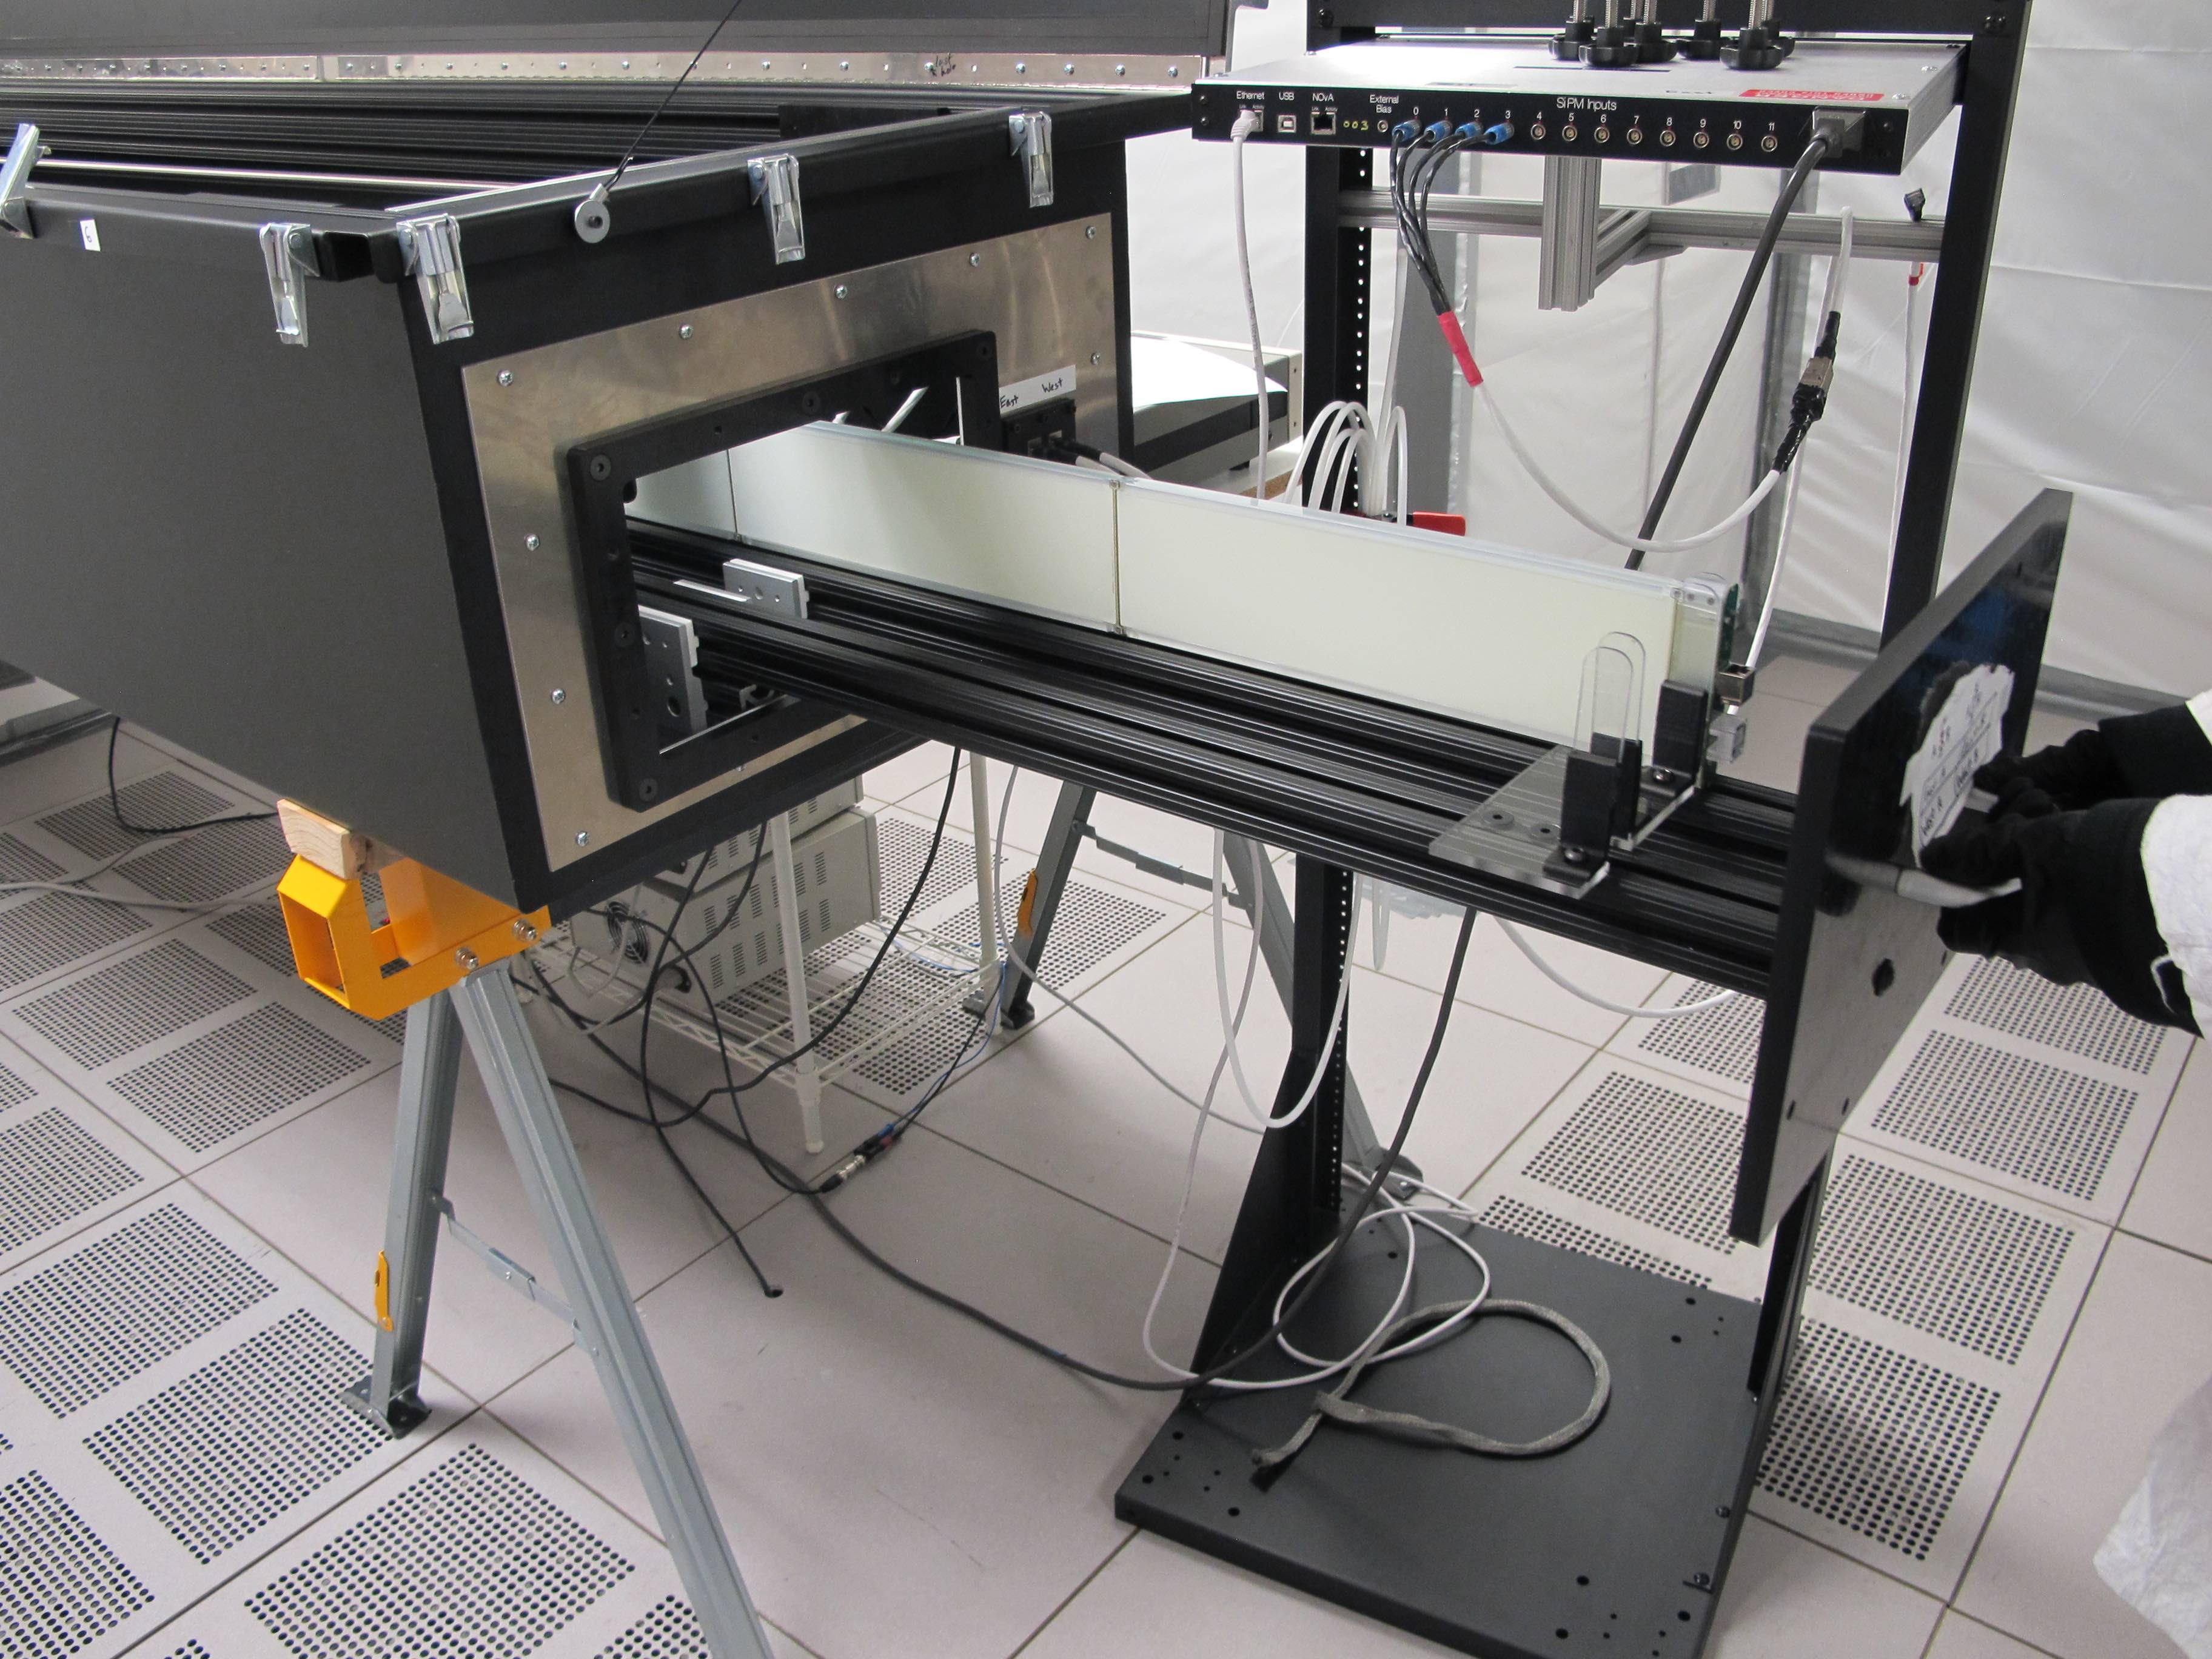
\includegraphics[width=0.4\columnwidth]{pds-pd-scanner.jpg}
\end{dunefigure}


%%%%%%%%%%%%%%%%%%%%%%%%%%%%%%%%%%
\subsection{APA Frame Mounting Structure and Module Securing}	
\label{sec:fdsp-pd-assy-frames}
%\todo{\color{blue} Content:  Warner}

\Dword{pd} modules are inserted into the \dword{apa} frames through ten slots 
(accessing five on each side of the \dword{apa} frame) and are supported inside the frame by 
stainless steel guide channels.  The slot dimensions for the \dword{pdsp} \dword{apa} frames 
are \SI{136.0}{mm}$\times$\SI{25.0}{mm}\footnote{For \dword{pdsp} they were only\SI{108.0}{mm}$\times$\SI{19.2}{mm} wide; the increase allowed for larger \dword{pd} modules and an increase in light collection area of nearly 50\% over the ProtoDUNE design.}   
(see Figure~\ref{fig:pds-pd-mounting}(left)).
The guide channels are pre-positioned into the \dword{apa} frame prior to applying the wire shielding mesh to the \dword{apa} frames, and are not accessible following wire wrapping. Following insertion, the \dword{pd} modules are fixed in place in the \dword{apa} frame using two stainless steel captive screws, as shown in Figure~\ref{fig:pds-pd-mounting}(right).
 
 \fixme{Dave W Will replace prior to second draft with similar but corrected images for current X-ARAPUCA design}

\begin{dunefigure}[\dword{pd} mounting rails in \dword{apa} frame.]{fig:pds-pd-mounting}
{\dword{pd} mounting in \dword{apa} frame: Rails (left) and securing to the frame with captive screws  (right).}
	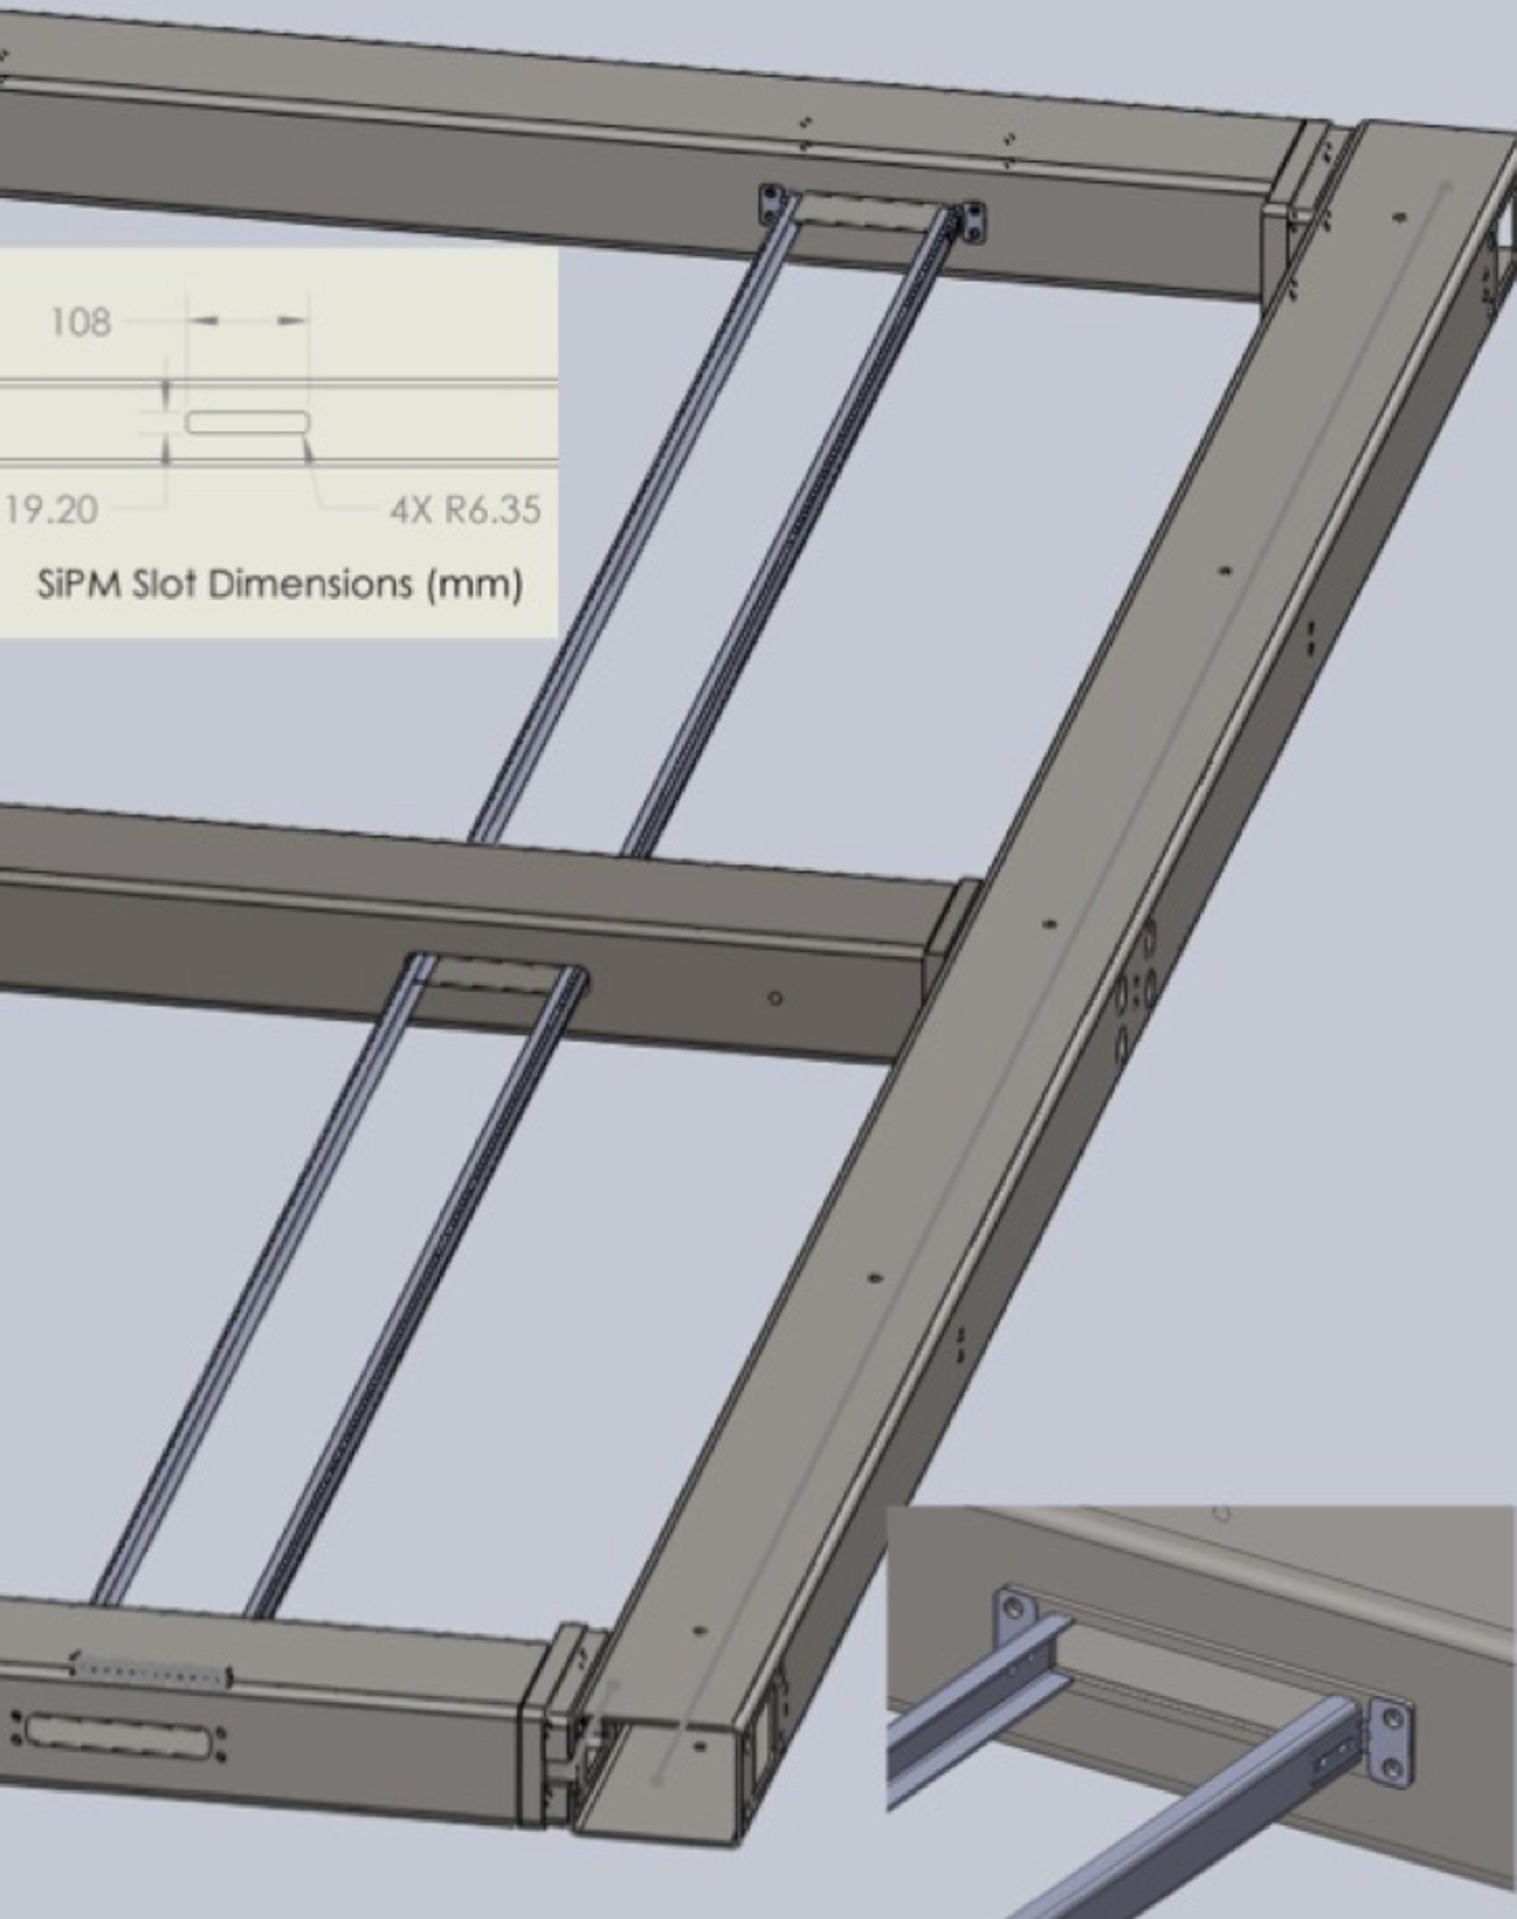
\includegraphics[height=7cm]{pds-pd-mounting-rails.pdf}
	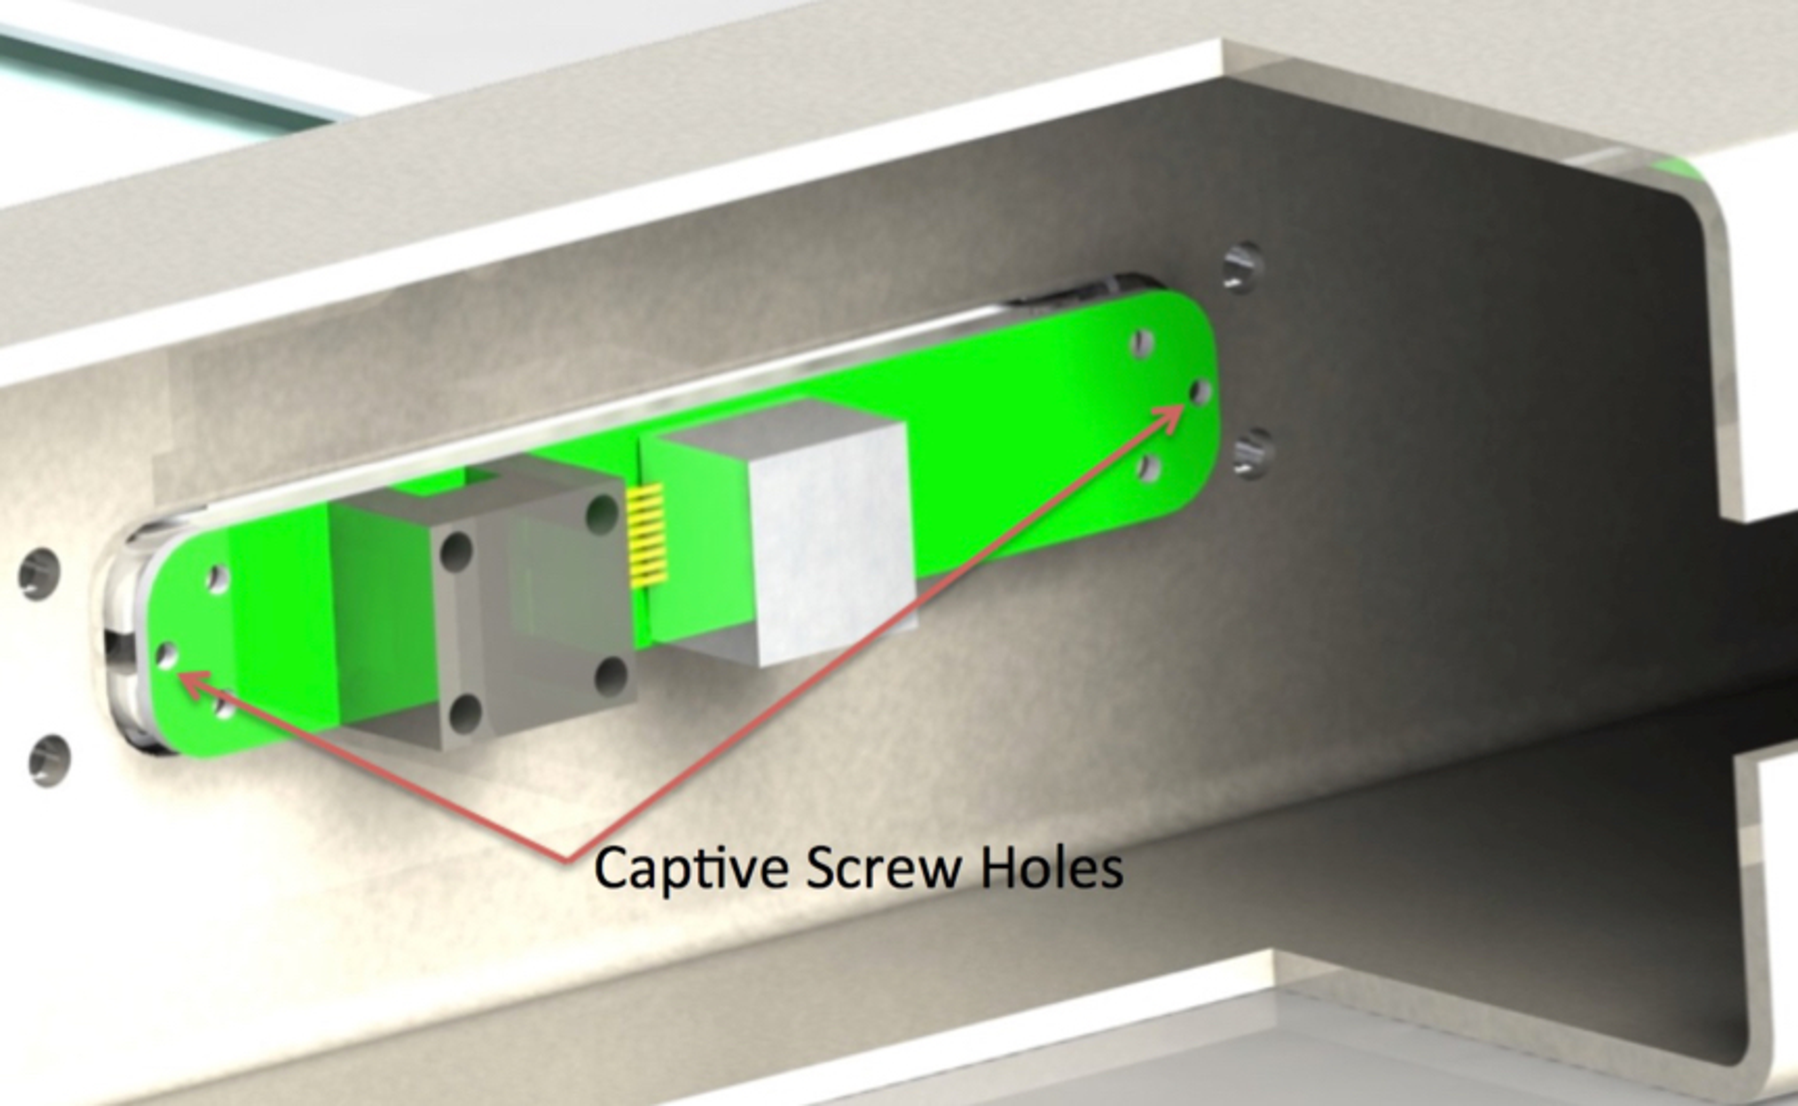
\includegraphics[height=5cm]{pds-pd-mounting-screws.pdf}
\end{dunefigure}

\subsubsection{Signal cable and connections}

For the \dword{pdsp} \dword{pds}, photon detector cables were run inside the APA side tubes, five cables per side.  For the far detector, however, this space will be filled by cold electronics cables.  This change required a revised plan for locating the PD cables.  In addition, it was observed during \dword{pdsp} \dword{pds} installation that running the PD cables and making electrical connections to the modules during PD integration was time consuming and introduced risk to the process.

For the far detector, the PD cables will be pre-positioned in the APA frames prior to installing the ground shield mesh and wire-wrapping the frame.  This will require two different styles of APA frame--  Those intended to be installed in the bottom position in an APA stack which will house the cables for only the lower APA and those intended to be installed in the top position, which will house the cables for both the upper APA PDs and the pass-through cables from the lower APA, all cables terminating at the header of the top APA after assembly (see Figure~\ref{fig:pd-cable-routing-APA-Frames}).

The cable connections between the upper and lower APAs is made during APA installation into the cryostat, while the APA stack is being fabricated.  The same in-line multi-pin connectors used at the flange penetration in \dword{pdsp}\footnote{Hirose LF 10WBP-12S connectors https://www.hirose.com} are used for this connection.
%\fixme{Dave: Do you want to put more specific info in the footnote on the connector?}

The PD signal cables are expected to thermally contract approximately 2\% during cool-down of the detector to cryogenic temperatures.  This is accounted for in the design by leaving cable loops in place between the anchor points to the APA frame, allowing for the required relative motion.

%\fixme{need to put in figures of cables in APA frames here}

\begin{dunefigure}[\dword{pd} cable routing in \dword{apa} frames.]
{fig:pd-cable-routing-APA-Frames}
{\dword{pd} cable routing in \dword{apa} frames: Bottom \dword{apa} (left) and top \dword{apa} (right).}
	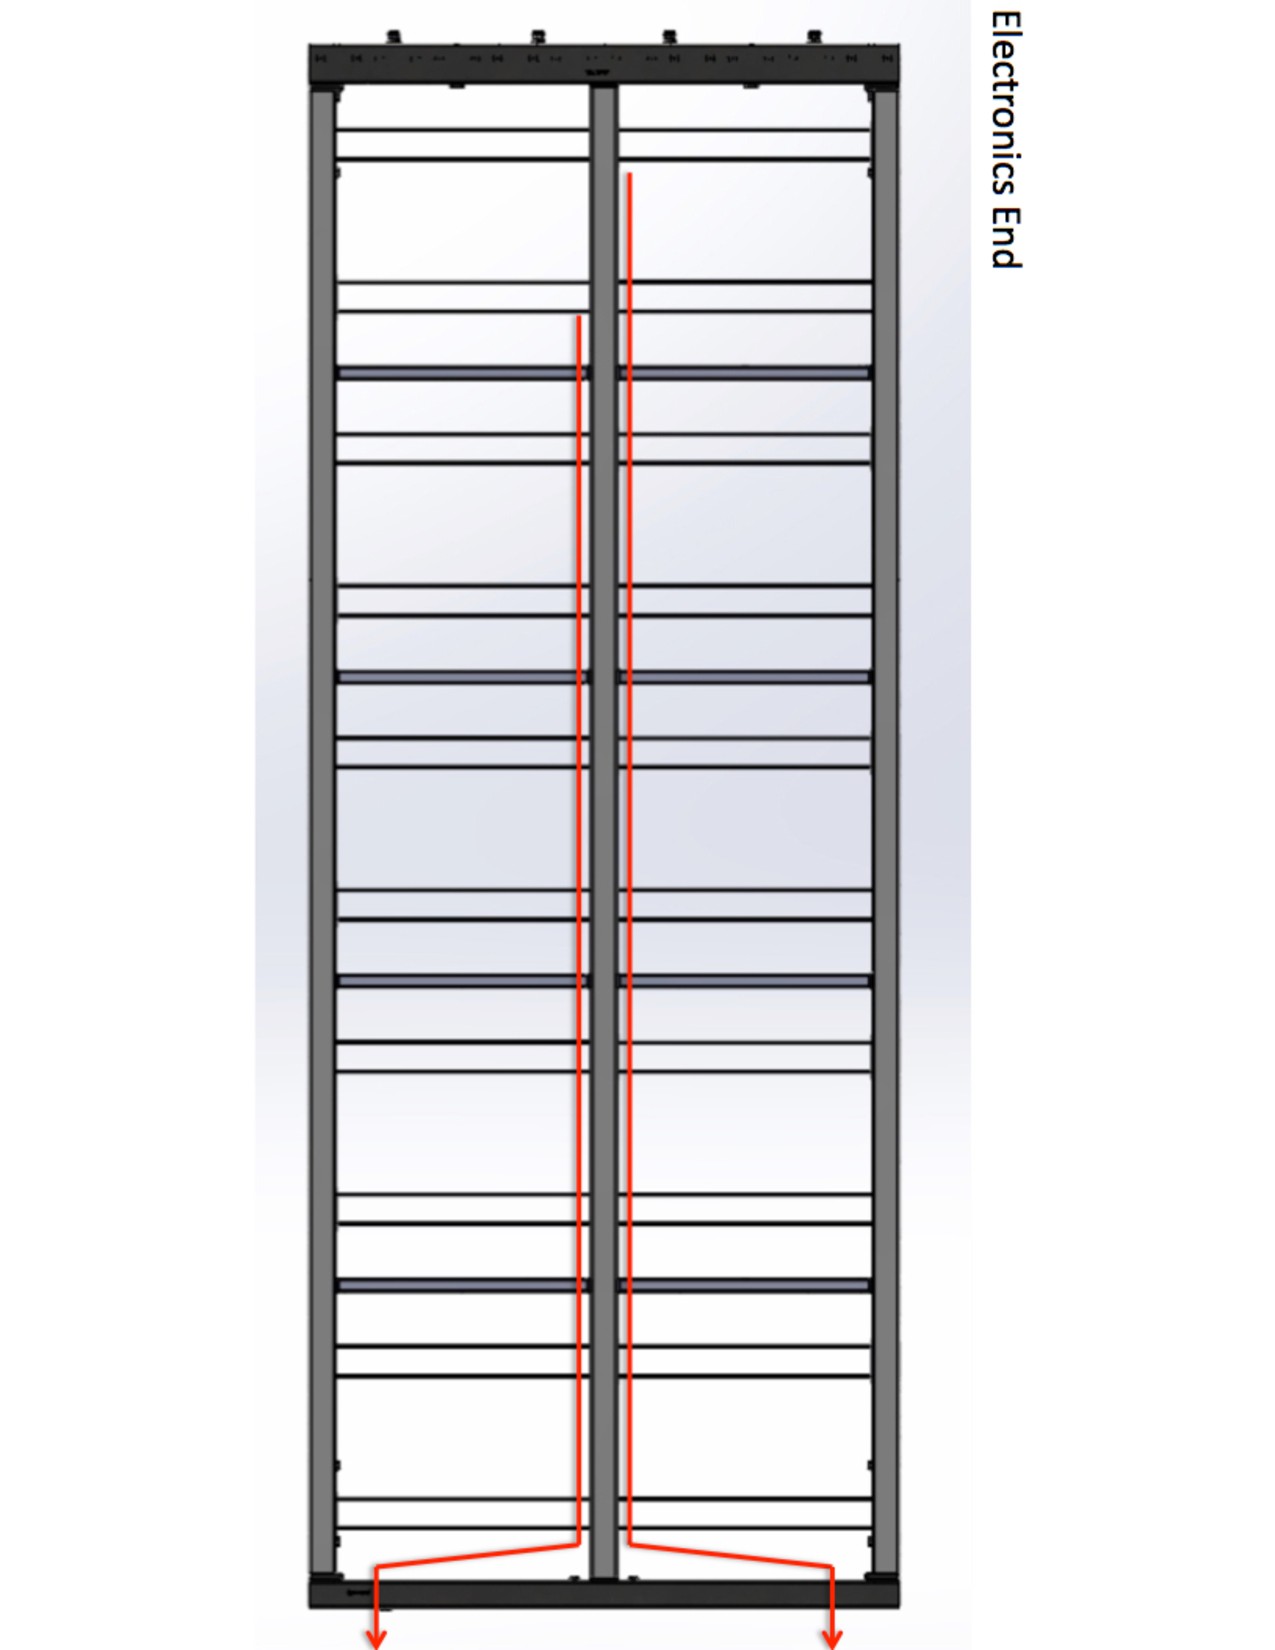
\includegraphics[angle=90,height=6.5cm]{pds-lower-apa-pds-cable-routing}
	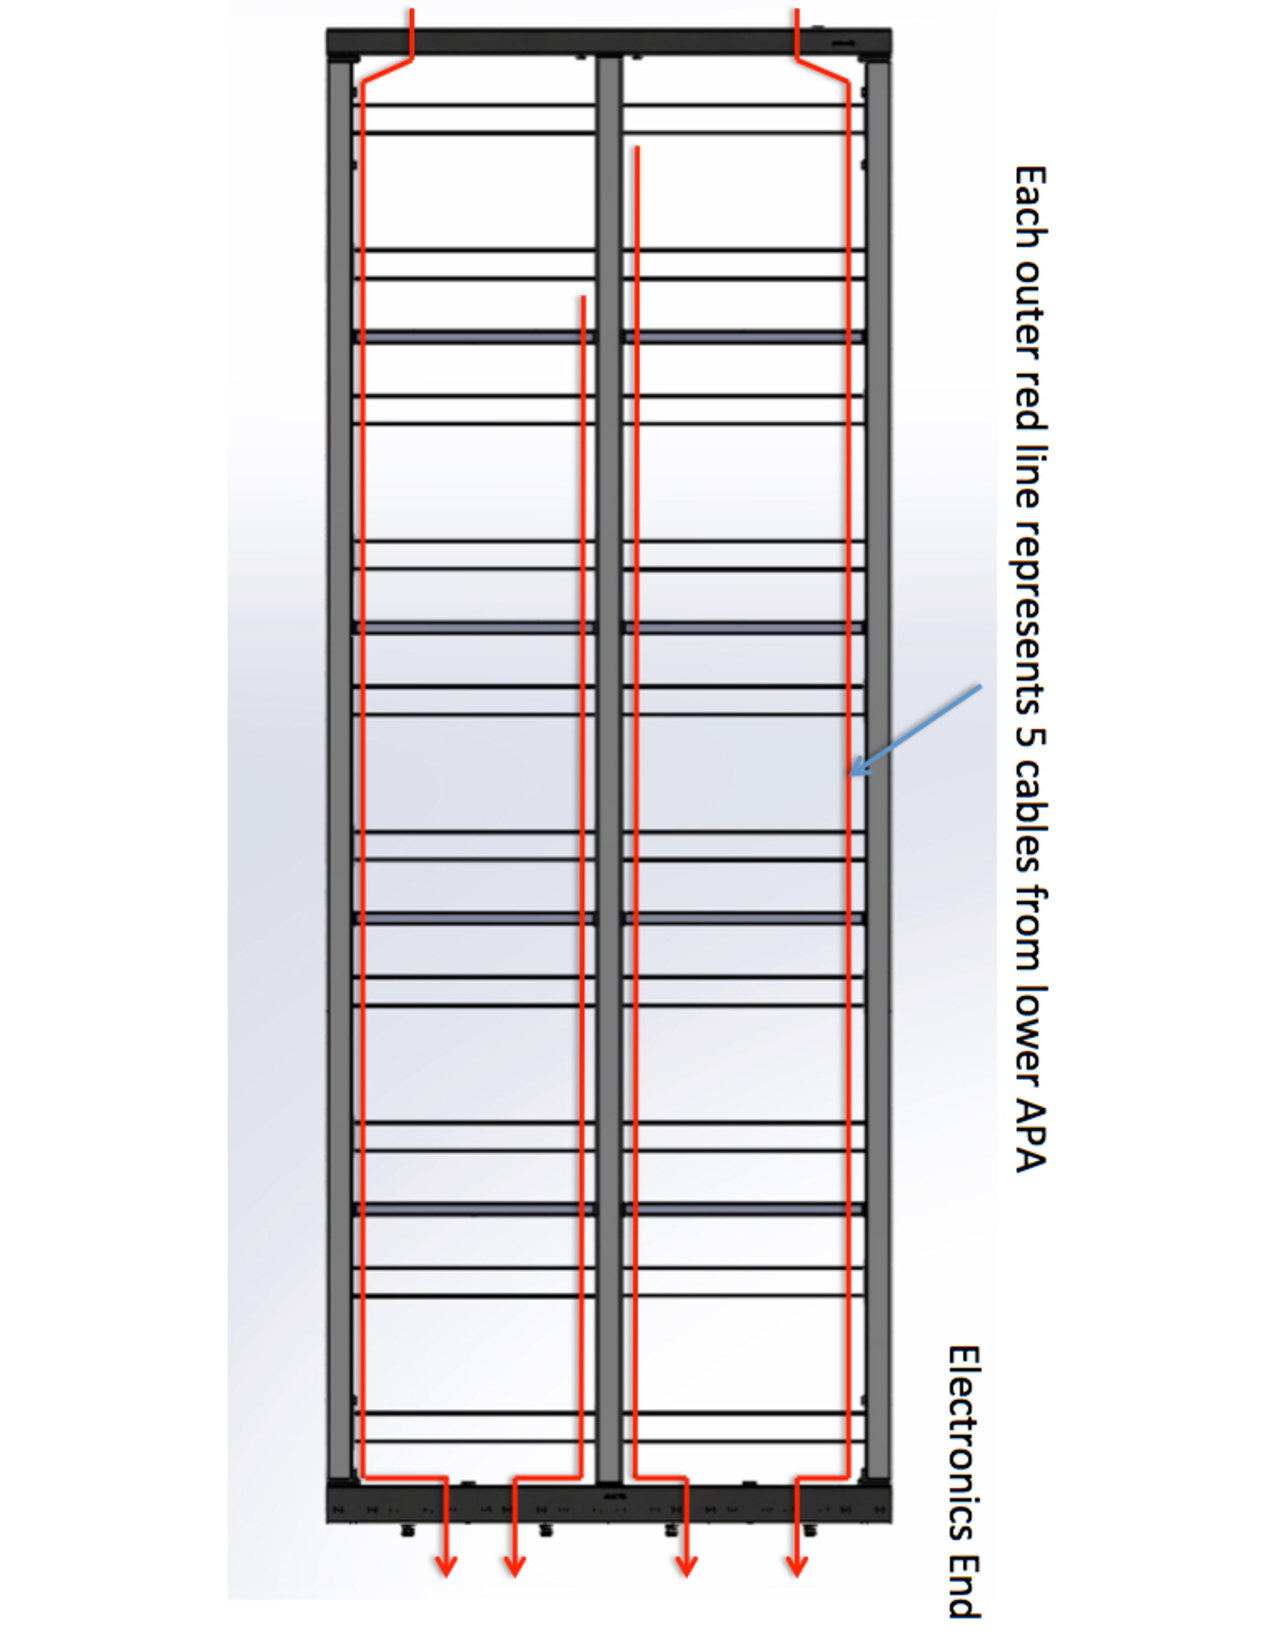
\includegraphics[angle=90,height=6.5cm]{pds-upper-apa-pds-cable-routing}
	\vspace{-1.5cm}
\end{dunefigure}

To remove interference with the CE cables, the electrical connections between the PD modules and the pre-positioned cable harness were moved to the face of the central APA tube.  Printed circuit boards with spring-loaded electrical sockets are pre-positioned on the inside face of the tube as part of the PD rail installation as shown in figure ~\ref{fig:pd cable connectors.} (left).  During PD integration into the APA frames, a PCB with pin contacts mounted to the PD module (See figure~\ref{fig:mounting-board-routing-board} right) engages into the PCB mounted to the APA frame, automatically making the electrical connection as shown in figure ~\ref{fig:pd cable connectors.} (right)

%\fixme{Dave: you have three figure references in the paragraph - I am not certain which goes with which so I will leave that for you.}

\begin{dunefigure}[\dword{pd} cable connectors.]{fig:pd cable connectors.}
{\dword{pd} cable connectors in \dword{apa} frames: PD connector plate mounted in APA frame (ICEBERG model, left) and installed PD/connector assembly in \dword{apa} (right).  Note that active ganging PCBs are buried inside the central tube.}
	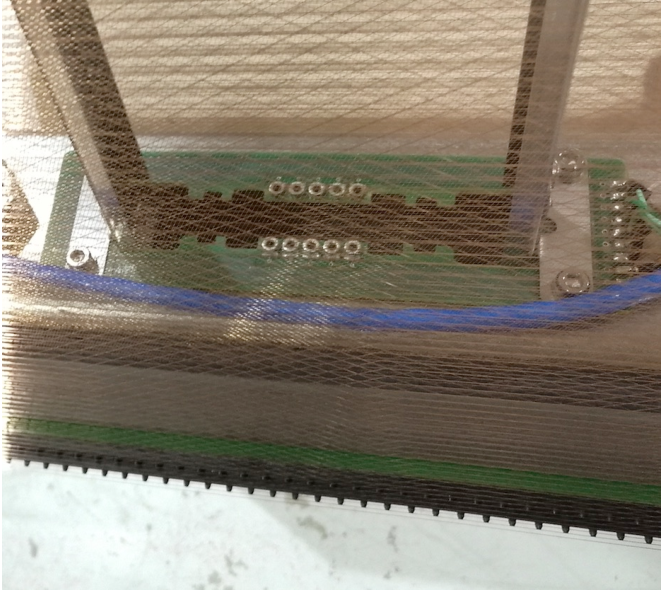
\includegraphics[height=7.5cm]{pds-connector-mounted-in-apa.pdf}
	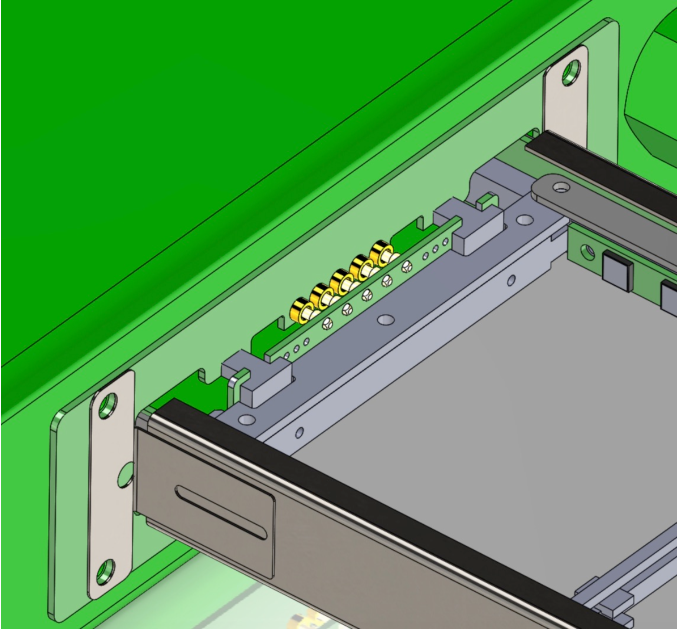
\includegraphics[height=7.5cm]{pds-connector-assembly-in-apa.pdf}
\end{dunefigure}

\subsubsection{Thermal Contraction and Load Deformation}

%\fixme{Should we demote the thermal contraction and deflections to a single subsection, of engineering calculations?}

\textit{\bf Thermal Contraction}

During cool down from room temperature to \dword{lar} temperatures, there is a possibility of significant relative shrinkage of module components.  Mitigating these effects was a major consideration in the X-ARAPUCA module design.

Thermal expansion coefficients (CTEs) for the stainless steel APA frames and fused-silica filter plates drove the materials selection for the ARAPUCA modules.  The frame components are fabricated from FR-4 G-10, resulting in a shrinkage of the stainless steel frame structure relative to the frame of approximately \SI{1.2}{mm} along the long ($\sim$\SI{2}{m}) axis of the bar.  The shrinkage of the frame relative to the filter plate is <\SI{0.2}{mm}.  Both these relative shrinkage factors are accounted for in the dimensions and tolerances of the design.

The largest relative contraction of mechanical components is between the FR-4 frame and the acrylic WLS plates. The most critical shrinkage is between the face of the photosensors and the WLS plate, where the \SI{92}{mm} width of the plate will result in an increase in separation between the sensor face and the WLS plate of approximately \SI{1.3}{mm}.  Studies are ongoing in simulation and testing to understand the impact this will have on the performance of the X-ARAPUCA.  Relative contraction along the long axis of the WLS plate (\SI{487.0}{mm} long plate, resulting in a \SI{5.8}{mm} relative contraction) is addressed by the WLS bar mounting structure.

\begin{dunetable}[Shrinkage of \dword{pd} materials.]
%{|c|c|}
{lc}
{tbl:fdsfpdshrink}
{Shrinkage of \dword{pd} module materials for a $206^{\circ}$C temperature drop}
Material 			 & Shrinkage Factor (m/m)\\ \toprowrule
Stainless Steel (304) & $2.7\times10^{-3}$\\ \colhline
FR-4 G-10 (In-plane) & $2.1\times10^{-3}$\\ \colhline
Fused Silica (Filter Plates) & $1.1\times10^{-4}$\\ \colhline
Acrylic (WLS Bars) & $1.4\times10^{-2}$\\ \colhline
\end{dunetable}

  Mitigation of these contractions is detailed in Table~\ref{tbl:fdsfpdshrinkeffects}.

\begin{dunetable}[Relative shrinkage of \dword{pd} components and \dword{apa} frame]
%{|p{0.2\textwidth}|p{0.2\textwidth}|p{0.5\textwidth}l}
{p{0.2\textwidth}p{0.2\textwidth}p{0.5\textwidth}}
{tbl:fdsfpdshrinkeffects}
{Relative Shrinkage of \dword{pd} components and \dword{apa} frame, and mitigations.}
\textbf{Interface} & \textbf{Relative shrinkage} & \textbf{Mitigation} \\ \toprowrule
\dword{pd} Length to \dword{apa} width & \dword{pd} expands  \SI{1.2}{mm} Relative to \dword{apa} frame & \dword{pd} affixed only at one end of \dword{apa} frame, free to expand at other end.  \SI{3}{mm} nominal clearance (beyond tolerance allowance) for expansion in design \\ \colhline
Width of \dword{pd} in \dword{apa} Guide Rails & \dword{pd} expands \SI{.1}{mm}  relative to slot width & \dword{pd} not constrained in C-channels. C channels and tolerances designed to contain module across thermal contraction range \\ \colhline
Width of \dword{sipm} mount board ({\it Hover board}) to stainless steel frame & Stainless frame shrinks \SI{0.1}{mm}  more than PCB & Diameter of shoulder screws and FR-4 board clearance holes selected to allow for motion \\ \colhline
Length of WLS bar relative to FR-4 \dword{pd} frame & WLS bar shrinks \SI{5.8}{mm} relative to PD frame & Allowed for in WLS bar mount fixtures \\ 
\end{dunetable}

%\subsubsection{\dword{pd} Mount frame deformation under static \dword{pd} load}

\textit{\bf \dword{pd} Mount frame deformation under static \dword{pd} load}

\fixme{Section will remain but requires new calculations based on X-ARAPUCA design.  Will be complete by January 2019 revision.}

\Dword{fea} modeling of the \dword{pd} support structure was conducted to study static deflection 
prior to building prototypes.  Modeling was conducted in both the vertical
 orientation (\dword{apa} upright, as installed in cryostat) and also horizontal orientation.  
Basic assumptions used were fully-supported fixed end conditions for the rails, 
with uniform loading of 3X \dword{pd} mass (\SI{5}{kg}) along rails.  
Figure~\ref{fig:pds-rail} illustrates the rail deflection for the \dword{apa} in the horizontal (left) and vertical (right) orientations.
Prototype testing confirmed these calculations.

\begin{dunefigure}[\dword{pd} mechanical support analysis.]{fig:pds-rail}
{\dword{pd} mechanical support analysis: Rail deflection for the \dword{apa} in the horizontal (left) and vertical (right) orientations.}
	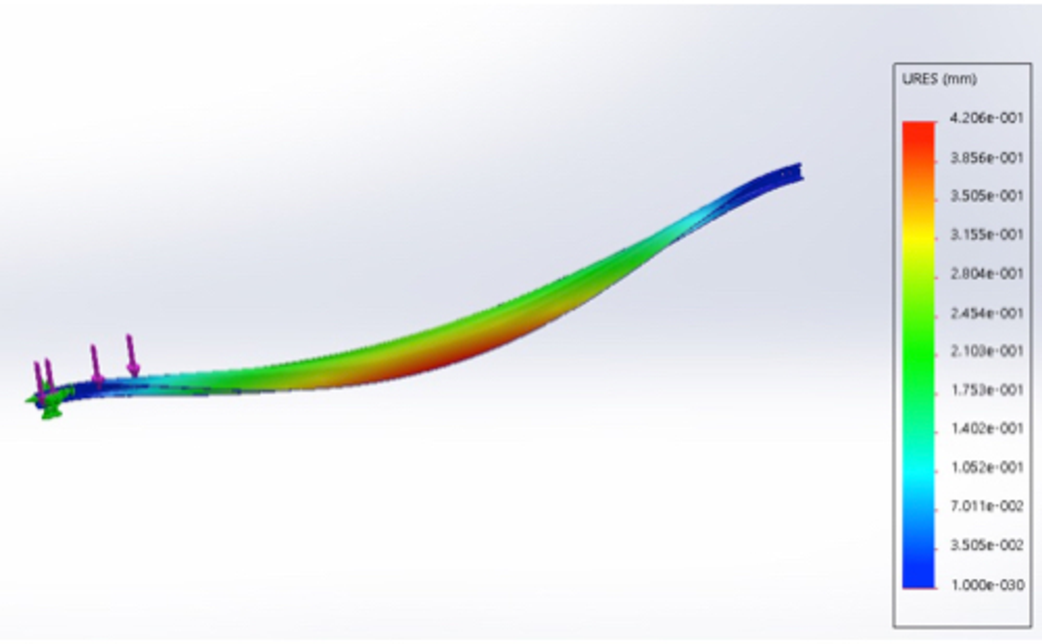
\includegraphics[height=4.5cm]{pds-rail-deflec-apa-flat.pdf} 
	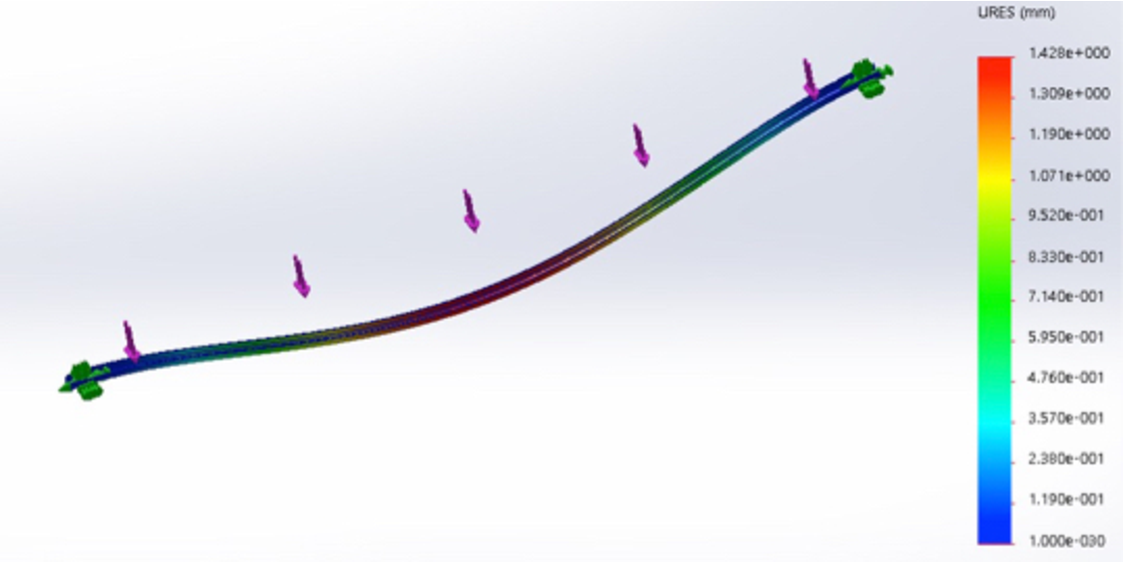
\includegraphics[height=4.5cm]{pds-rail-deflec-apa-vert.pdf}\\
%	%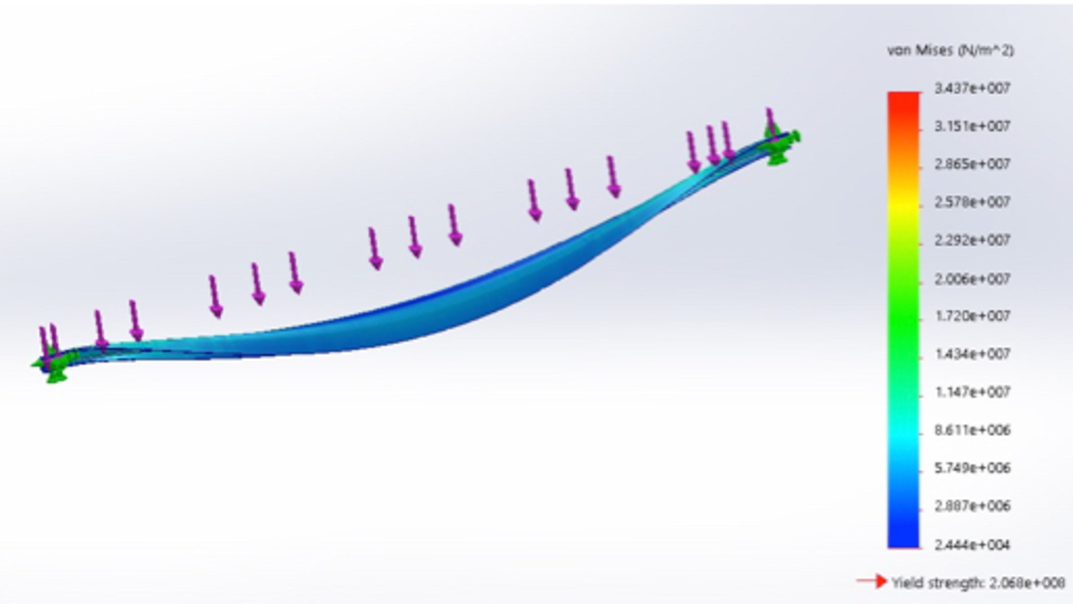
\includegraphics[width=0.25\columnwidth]{pds-rail-stress-apa-flat.pdf} 
%	%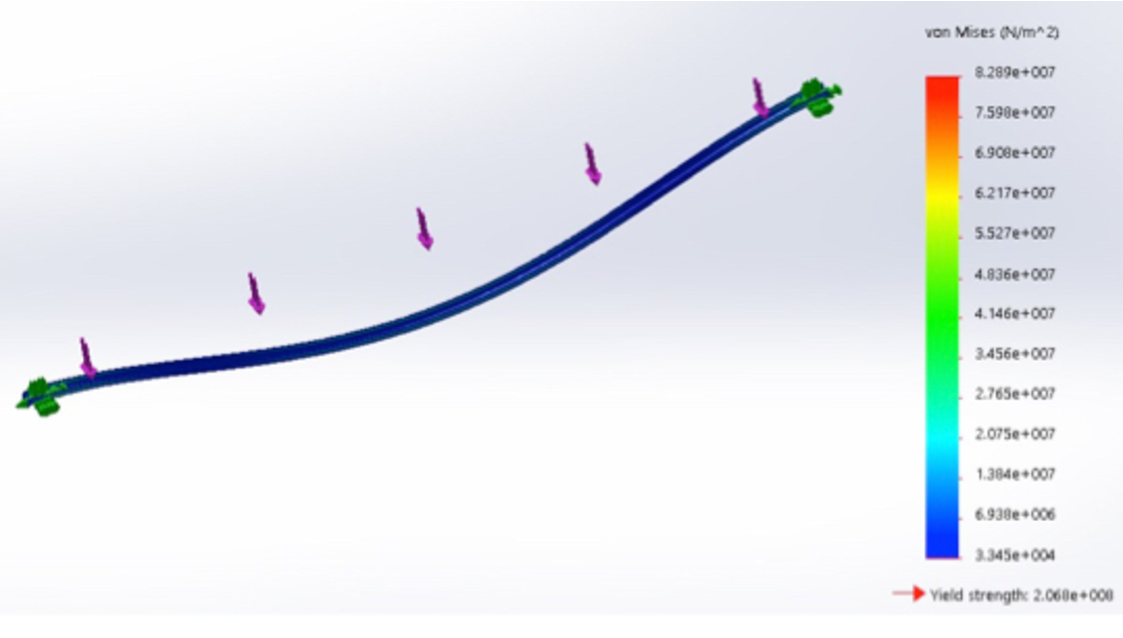
\includegraphics[width=0.25\columnwidth]{pds-rail-stress-apa-vert.pdf}
\end{dunefigure}


%%%%%%%%%%%%%%%%%%%%%%%%%%%%%%%%%%
\subsection{Photosensors and Photosensor Modules}
\label{sec:fdsp-pd-assy-psm}
%\metainfo{\color{blue} Content: Zutshi/Cancelo/Moreno?}

The use of SiPMs in noble liquids is relatively young but rapidly growing field with experiments such as GERDA, MEG II, Darkside, nEXO etc. in various stages of preparation. DUNE will learn immensely from their experience but in principle imposes even more stringent accessibility and longevity constraints. Risk mitigation through reliability engineering, process control and both vendor and Collaboration testing will be a key feature of the DUNE SiPM production process.

{\it{Reliability Engineering:}} The primary issue is the changes in material properties and thermal stresses induced in the packaging due to differential coefficients of thermal expansions (CTEs). This is especially critical for interfaces with the relevant ones in this case being die-to-substrate, substrate-to-potting mold, potting mold-to-encapsulation and solder joints-to-everything else. Analysis of these interfaces and collaboration with vendors to match CTEs as far as possible at these interfaces will contribute substantially to the long-term reliability of the photosensor.

{\it{Process Control:}} Small and superficially innocuous seeming changes in the fabrication process of the photosensors can have a big impact on the robustness of these devices at extreme temperatures. This is one of the reasons why in space applications, for instance, same-day same-batch components are utilized. Given the photosensor quantities involved, this criteria is not a practical option for the DUNE PDS but does imply an MoU with the vendor in terms of strict process control once the pre-production batch has been qualified.

{\it{Quality Assurance:}} This will be an essential component in the photosensor risk mitigation strategy consisting of restricting the number of production batches, clearly communicating desired device and packaging parameters to the vendor and vendor testing to warrant device operation down to liquid nitrogen temperatures. This requirement implies that, before shipment to the Collaboration, the vendor will qualify a randomly selected sample of devices from each production batch. The qualification would entail thermally stressing the devices and before/after visual and electrical measurements. 

{\it{Quality Control:}} The above strategies, while significantly lowering the risk, will not obviate the need for a strict testing regimen. Every sensor will be tested multiple times, at various stages of assembly, before installation in the detector.

\Dwords{sipm} will be mounted in groups of six passively-ganged sensors to mounting boards, with eight mounting boards per supercell.  Passive ganging (sensors in parallel) is implemented with traces on the \dword{sipm} mounting board (module) and has been implemented for \dword{pdsp}.  The \dwords{sipm} are mounted using a pick-and-place machine and standard surface mount device soldering procedures. The outputs from these mounting boards are then routed to active ganging circuits in the center of the PD module, where they are collected into a summing amplifier and reduced to a single output channel.

%\fixme{Is the following a Production and Assembly topic?}
%\fixme{Dave W--  I think this should stay here--  it is a design feature}
% rjw 21/4/18 ok

The ganged analog signals are then brought out via long cables (approximately \SI{25}{m}) for digitization outside the cryostat.
\dword{pdsp} has provided essential operational experience with a passive ganging board and signal transport provided by Teflon ethernet CAT6 cables.
R\&D is needed to optimize the connectors used to couple the cable to the board;  it is a priority to understand the mechanical stresses involved in the \dword{sipm}-PCB-Connector system (with different CTEs) as it is cooled (or cycled) to cryogenic temperatures.


%%%%%%%%%%%%%%%%%%%%%%%%%%%%%%%%%%
\subsection{Electronics}
\label{sec:fdsp-pd-assy-pde}
%\metainfo{\color{blue}  Content: Moreno/Franchi/Djurcic}

Extensive experience of manufacturing processes was gained during the development of the SSPs used on \dword{pdsp}, a general description of the readout system of \dword{pdsp} can be seen in the Section~\ref{sec:fdsp-pd-pde}. Compatibility between elements designed by different institutions is guaranteed when standard procedures are followed, so the circuit design must be done in accordance with mutually agreed-upon specification documents.  A sufficient  number of units needs to be produced to allow local testing and for testing in the central facility -- for example, in \dword{pdsp} \num{5} 12-channel  SSPs were produced and delivered to CERN for integration testing. Twenty-four were fabricated for \dword{pdsp} operation. 

The readout electronics of the photon detection system will be designed and produced with similar tools and protocols used for  \dword{pdsp}. For example: printed circuit board (PCB) layout is performed in accordance with IPC\footnote{IPC\texttrademark{}, Association Connecting Electronics Industries, \url{http://www.ipc.org/}.} specifications. Bare PCB manufacturing requirements are embedded within the Gerber file fabrication documents (e.g., layers, spacing, impedance, finish, testing, etc.). Components are assembled on to circuit boards using either trained \dword{pd} consortium technical staff or by external assembly vendors, based upon volume, in accordance with per-design assembly specification documents. Testing occurs at labs and universities within the collaboration in accordance with a per-design test procedure that typically includes a mix of manual, semi-automatic and automated testing in an engineering test bench followed by overall characterization in a system- or subsystem-test stand.
Other considerations and practices relevant to readout electronics production and assembly are itemized here:

\begin{itemize}

\item Components: Schematic capture is done using appropriate tools (such as OrCAD 16.6.\footnote{OrCAD\texttrademark{} schematic design tool for PCB design http://www.orcad.com} or similar toolset) available within design facility. Design is hierarchical with common front-end page referenced multiple times to ensure that all input channels are identical. The schematic contains complete bill-of-materials (BOM) including all mechanical parts. A subversion repository or similar tools are typically used for version control and backup. Multiple internal design reviews held before schematic is released to layout. The bill of materials is stored directly within schematic, extracted to spreadsheet when ordering parts. Every part is specified by both manufacturer and distributor information. Distributor information may be overridden by a technician at order time due to price or availability. Standard search engines such as Octopart\footnote{Octopart https://octopart.com/}, ECIA\footnote{ ECIA https://www.eciaauthorized.com} and PartMiner\footnote{PartMiner https://www.part-miner.com/} are used to check price or availability across all standard distributors. A parts availability check review is performed prior to handoff from schematic to layout; as required obsolete or long lead time parts were removed from design and replaced. BOM information will include dielectric, tolerance, temperature coefficient, voltage rating and size (footprint) to ensure all parts are fully described.

\item Boards: There are standard tools (such as the Allegro\footnote{Cadence Allegro\textregistered PCB design solution https://www.cadence.com} toolset) available for the printed-circuit-board (PCB) layout. Conventional PCBs are realized as multi-layer boards with controlled impedance with many sets of delay-matched nets where necessary. In usual practice the complete impedance and delay characteristics are calculated within layout tool and crosschecked by PCB vendor prior to manufacture. In usual practice, a competitive bid between multiple previously qualified vendors is used, with a full electrical and impedance testing required. Multiple internal design reviews are held prior to release of the design.

\item Cable plant: Cabling will be designed taking into consideration the \dword{apa} space and in close collaboration with the TPC electronics group to avoid cross-talk effects. A final decision on cable procurement will be taken based on the possibility of cable manufacturing in an institution belonging to the photon detection consortium and the cost of a commercial solution.  

\item Manufacturer list: In addition to the general laboratory procedures for quality assurance, the general practice will be to use only printed circuit board manufacturers and external assembly vendors whose workmanship and facilities have been personally inspected by experienced production team members. All external assemblers are required to quote in accordance with an assembly specifications document describing the IPC class and specific solder chemistry requirements of the design. The bill of materials document will show selected and alternate suppliers where available for every component of the front-end boards.

\item Front-end (FE) electronics firmware: This will be specified and updated iteratively in collaboration with other systems. The electronics working group will be responsible for responding to requests for additional firmware development, including for example, modifications to timing interface, modifications to trigger interface, and implemented sensitivity to in-spill vs. not-in-spill conditions. Documents describing firmware architecture for each major change will be written and distributed to \dword{pd} and DAQ working groups before implementation. \Dword{fe}  electronics user's manual containing all details of new firmware will be distributed with production units when manufactured.

\item Mechanical assembly: With the mechanical assembly of electronics readout boards it is common practice to use a 3D model generated by the layout software.  %AutoCAD\footnote{AutoDESK AutoCAD\textregistered computer aided design software application https://www.autodesk.com/} or similar software with Allegro (as PCB layout tool). 
All relevant dimensions of the PC board including connector and indicator placement is extracted as a base DXF file from which overall exploded mechanical diagram of chassis and other mechanical parts is made.  Mechanical items such as shield plates will be provided as well. It is assumed that the front-end chassis will made by external vendors (one for chassis, one for front/back panels) from drawings provided by the consortium.

\end{itemize}

\subsection{Calibration and Monitoring}
\label{sec:fdsp-pd-assy-CandM}
%\metainfo{\color{blue}  Content: Djurcic}

Extensive experience of manufacturing, testing and assembly processes was gained during the development of the calibration/monitoring system for \dword{pdsp}.
A general description of the proposed calibration and monitoring system can be seen in the Section~\ref{sec:fdsp-pd-CandM}. 

The design and production of the Calibration Modules with electronics circuitry, with FPGA implementation for light source controls and with optical timing/trigger and DAQ communication protocols, with implementation of UV light sources, follows closely the process described in Section~\ref{sec:fdsp-pd-assy-pde}.

Design and selection of cold diffuser components and selection of cold and warm quartz fiber components follows requirements derived from interface considerations with HV/CPA and Cryostat systems, and was tested in \dword{pdsp}.
Installation and QA/QC of optical fibers is performed during the CPA installation process with diffusers and CPA fibers pre-installed with CPAs.

Installation of fibers that connect CPA's fiber connections to the optical feed-through penetrations at cryostat will be defined with DSS and cryostat teams, based on installation experience in \dword{pdsp}. 
